\documentclass[a4paper,oneside,article]{memoir}



% LAYOUT
\usepackage{changepage}
\setulmarginsandblock{0.7\uppermargin}{0.8\lowermargin}{*}

% MATHS
\usepackage{amsmath,amsfonts,amssymb,amsbsy,commath,mathtools,calc}
\mathtoolsset{showonlyrefs,showmanualtags}

\usepackage{subfig}
% FONTS & LANGUAGE
\usepackage[usenames,dvipsnames]{color}
\definecolor{light-gray}{gray}{0.8}
\usepackage{fontspec,xltxtra,polyglossia}
\setmainlanguage{english}
\usepackage[normalem]{ulem} % have underlinings work
%\defaultfontfeatures{Ligatures=TeX}
\defaultfontfeatures{Mapping=tex-text}

\setmainfont[Ligatures={Common}, Numbers={OldStyle}]{Linux Libertine O}
%\setmainfont{Droid Sans}
%\setsansfont[Scale=MatchLowercase]{Inconsolata}
\setmonofont[Scale=0.8]{DejaVu Sans Mono}

% PDF SETUP
\usepackage[unicode,bookmarks, colorlinks, breaklinks,
pdftitle={T-61.5140: Prerequisites},
pdfauthor={Ville Väänänen},
pdfproducer={xetex}
]{hyperref}
\hypersetup{linkcolor=black,citecolor=black,filecolor=black,urlcolor=MidnightBlue} 

% TABLES
\usepackage{booktabs}
\usepackage{topcapt} 
\usepackage{rccol}
\usepackage{tabularx} % requires array
\newcommand{\otoprule}{\midrule[\heavyrulewidth]}
\newcolumntype{d}[2]{R[.][.]{#1}{#2}}

\usepackage{titlesec}

%%%%%%%% OMAT KOMENNOT %%%%%%%%%%%%

\usepackage{mymath}
\usepackage{mylayout}



% PARAGRAPHS
%\usepackage{parskip}

% kuvat

\usepackage{listings}
\usepackage{mcode}
\lstset{ %
	%language=Matlab,                % choose the language of the code
	basicstyle=\footnotesize\ttfamily,% the size of the fonts that are used for the code 
	numbers=none,                   % where to put the line-numbers
	numberstyle=\footnotesize\ttfamily,      % the size of the fonts that are usedfor the line-numbers 
	stepnumber=5,                   % the step between two line-numbers. If it's 1 each line 
	aboveskip=2\medskipamount,
	belowskip=2\medskipamount,                                % will be numbered
	numbersep=-5pt,                  % how far the line-numbers are from the code
	backgroundcolor=\color{white},  % choose the background color. You must add \usepackage{color}
	showspaces=false,               % show spaces adding particular underscores
	showstringspaces=false,         % underline spaces within strings
	showtabs=false,                 % show tabs within strings adding particular underscores
	frame=l,
	framesep=0pt,
	framexleftmargin=2mm,
	rulecolor=\color{light-gray},	                % adds a frame around the code
	tabsize=2,	                % sets default tabsize to 2 spaces
	caption=,
	captionpos=t,                   % sets the caption-position to bottom
	breaklines=true,                % sets automatic line breaking
	breakatwhitespace=false,        % sets if automatic breaks should only happen at whitespace
	emptylines=*1,
	%title=\lstname,                 % show the filename of files included with
	                                % also try caption instead of title
	escapeinside={\%*}{*)},         % if you want to add a comment within your code
            % if you want to add more keywords to the set
}

\newcommand{\course}{S-114.4202}
\newcommand{\coursename}{Special Course in Computational Engineering II}
\newcommand{\duedate}{\today}
\newcommand{\studentid}{63527M}
\renewcommand{\title}{Exercise Report}
\author{Ville Väänänen}

\setsecnumdepth{subsubsection}
\counterwithout{section}{chapter}
%\counterwithout{subsubsection}{section}
%\counterwithout{subsubsection}{subsection}
%\renewcommand\thesection{\arabic{section}}
\checkandfixthelayout
\renewcommand{\thesubsubsection}{\thesubsection{\large\scshape\alph{subsubsection}}}
\newfontfamily\subsubsectionfont[Letters=SmallCaps]{Linux Libertine O}
\titleformat{\subsubsection}{\large\scshape}{\alph{subsubsection} )}{10pt}{}
\titleformat{\section}{\Huge}{Round \thesection}{10pt}{}
\titleformat{\subsection}{\Large}{Exercise \thesubsection}{10pt}{}

\everymath{\displaystyle}
\begin{document}

\begin{titlingpage}
	\begin{adjustwidth}{-0.6in}{-0.6in}
	\begin{center}
		%\begin{minipage}{1.2\textwidth}
			\begin{flushright} \large
			Ville \textsc{Väänänen}\\
			\studentid\\
			ville.vaananen@aalto.fi
			\end{flushright}
		%\end{minipage}
		\vspace{8.0cm}
		
		\textsc{\LARGE \title}
		\HRule \\[0.19cm]
		{\large \course\: \coursename}
		
		\vfill
		\today
	\end{center}
	\end{adjustwidth}
\end{titlingpage}
\newpage


\section{}
\subsection{}
\subsubsection{}

The problem can be written in matrix form as follows:
\begin{align*}
	\v{y} &= \begin{bmatrix} y_1 & \dots & y_n \end{bmatrix}^T \\
	\v{a} &= \begin{bmatrix} a_1 & a_2 \end{bmatrix}^T \\	
	\v{X} &= \begin{bmatrix} 
				x_1 & 1 \\
				\vdots & \vdots \\
				x_n & 1 
%			 \end{bmatrix}^T \\
	\end{bmatrix} \\
	\v{y} &= \v{Xa}
\end{align*}

\subsubsection{}

\begin{align*}
	\mathrm{E}(a_1,a_2)&=(\v{y}-\v{Xa})^T(\v{y}-\v{Xa})
\end{align*}

\subsubsection{}
To compute the LS-estimate $\hat{\v{a}}$, we need to find the global minimum of $\mathrm{E}$, which can be
found by setting its gradient to zero (it's a quadratic form):
\begin{align}
	\nabla\mathrm{E}&=-2\v{X}^T(\v{y}-\v{Xa})\\
	&=2\v{X}^T\v{X}\v{a}-2\v{X}^T\v{y} \\
	\Rightarrow \hat{\v{a}} &= (\v{X}^T\v{X})^{-1}\v{X}^T\v{y}
\end{align}

\subsection{}
\subsubsection{}

The second order differential equation can be written as a first order vector valued differential equation as follows:
\begin{align}
	\dod{\v{x}(t)}{t}&=
	\begin{bmatrix}
	0&-c^2\\
	1&0
	\end{bmatrix}
	\begin{bmatrix}
	x'(t)\\
	x(t)
	\end{bmatrix}
	+
	\begin{bmatrix}
	1\\
	0
	\end{bmatrix}
	w(t)\\
	\Leftrightarrow\v{x}'(t)&=\v{F}\v{x}(t)+\v{L}w(t).
\end{align}
Let us proceed to solve this equation:
\begin{align}
	\v{x}'(t)-\v{F}\v{x}(t)&=\v{L}w(t)\\
	e^{-\v{F}t}\v{x}'(t)-e^{-\v{F}t}\v{F}\v{x}(t)&=e^{-\v{F}t}\v{L}w(t)\\
	\dod{}{t}\left(e^{-\v{F}t}\v{x}(t)\right)&=e^{-\v{F}t}\v{L}w(t)\shortintertext{so that}\\
	\v{x}(t)&=e^{\v{F}(t-t_0)}\v{x}(t_0)+\defint{t_0}{t}{e^{\v{F}(t-s)}\v{L}w(s)}{s} \label{eq:contsol}\shortintertext{where}\\
	\v{x}(t_0)&=
	\begin{bmatrix}
	v_0\\
	x_0
	\end{bmatrix}
\end{align}

\subsubsection{}
% After discretizing the time into $n+1$ instants as $\{t_0=0,t_1=\Delta t,\dots,t_n=n\Delta t\}$
% we can approximate \eqref{eq:contsol} as
% \begin{align}
% 	\v{x}(t_k)=\v{x}(t_{k-1}+\Delta t)&= \v{x}_0e^{\v{F}t_{k-1}}e^{\v{F}\Delta t}+\v{L}\Delta t\sum_{j=1}^{k}e^{\v{F}(t_{k-1}+\Delta t-t_{j-1})}w_{j-1}
% \end{align}
% where we have approximated the integral with its Riemannian sum and $w_{j-1}=w(t_{j-1})$.
% This can be further simplified into
% \begin{align}
% 	\v{x}(t_k)&= e^{\v{F}\Delta t}\left(\v{x}_0e^{\v{F}t_{k-1}}+\v{L}\Delta t\sum_{j=1}^{k-1}\left(e^{\v{F}(t_{k-1}-t_{j-1})}w_{j-1}\right) + \v{L}\Delta tw_{k-1}\right)\\
% 	&=e^{\v{F}\Delta t}\v{x}(t_{k-1}) + \v{L}\Delta t e^{\v{F}\Delta t} w_{k-1}
% \end{align}

After discretizing the time into $n+1$ instants as $\{t_0=0,t_1=\Delta t,\dots,t_n=n\Delta t\}$ and assuming $w(s)=w(t_{k-1})\; \forall s\in[t_{k-1},t_k)$
we can write \eqref{eq:contsol} as
\begin{align}
	\v{x}(t_k)&=e^{\v{F}(t_k-t_0)}\v{x}(t_0)+\sum_{j=1}^k \defint{t_{j-1}}{t_j}{e^{\v{F}(t_j-s)}\v{L}w(s)}{s}\\
	&=e^{k\v{F}\Delta t}\v{x}(t_0)+\sum_{j=1}^k \defint{t_{j-1}}{t_j}{e^{\v{F}(t_j-s)}}{s}\v{L}w(t_{j-1})\\
	&=e^{k\v{F}\Delta t}\v{x}(t_0)+\sum_{j=1}^k (-\v{F}^{-1})\left(1-e^{\v{F}\Delta t}\right)\v{L}w(t_{j-1})\\
	&=e^{k\v{F}\Delta t}\v{x}(t_0)+\v{F}^{-1}(e^{\v{F}\Delta t}-1)\v{L}\sum_{j=1}^k w(t_{j-1})\\
	%&=e^{\v{F}\Delta t}e^{\v{F}(k-1)\Delta t}\v{x}(t_0)+\v{F}^{-1}(e^{\v{F}\Delta t}-1)\v{L}\sum_{j=1}^{k-1} w(t_{j-1})+\v{F}^{-1}(e^{\v{F}\Delta t}-1)\v{L}\v{L} w(t_{k-1})\\
	&=e^{\v{F}\Delta t}\v{x}(t_{k-1})+\v{F}^{-1}(e^{\v{F}\Delta t}-1)\v{L} w(t_{k-1})\\
	&=\v{A}\v{x}(t_{k-1})+\v{B}w(t_{k-1})
\end{align}

% After discretizing the time into $n+1$ instants as $\{t_0=0,t_1=\Delta t,\dots,t_n=n\Delta t\}$ and assuming $w(s)=w(t_{k-1})\; \forall s\in[t_{k-1},t_k)$
% we can write \eqref{eq:contsol} for a single interval $[t_{k-1},t_k]$ as
% \begin{align}
% 	\v{x}(t_k)&=e^{\v{F}\Delta t}\v{x}(t_{k-1})+\defint{t_{k-1}}{t_k}{e^{\v{F}(t_k-s)}\v{L}w(s)}{s}\\
% 	&=e^{\v{F}\Delta t}\v{x}(t_{k-1})+\defint{t_{k-1}}{t_k}{e^{\v{F}(t_k-s)}}{s}\v{L}w(t_{k-1})\\
% 	&=e^{\v{F}\Delta t}\v{x}(t_{k-1})+(-\v{F}^{-1})\left(1-e^{\v{F}\Delta t}\right)\v{L}w(t_{k-1})\\
% 	&=e^{\v{F}\Delta t}\v{x}(t_{k-1})+\v{F}^{-1}(e^{\v{F}\Delta t}-1)\v{L}w(t_{k-1})\\
% 	&=\v{A}\v{x}(t_{k-1})+\v{B}w(t_{k-1})\\		
% \end{align}

\subsubsection{}

Assuming $w_{k-1}\sim N(0,\frac{q_c}{\Delta t})$ and that at each timestep $t_k$ we measure 
the value of $x(t_k)$ and additive zero mean gaussian noise with variance $R_k$ and designating 
$\v{x}_k=\v{x}(t_{k})$ we get the following linear Gaussian state space model:

\begin{align}
	%\v{x_k}&=\begin{bmatrix} 1 & e^{-c^2\Delta t}\\ e^{\Delta t} & 1 \end{bmatrix}\v{x}_{k-1}+\begin{bmatrix} 0 \\ -c^{-2}\left(e^{-c^2\Delta t}-1\right) \end{bmatrix}w_{k-1}\\
	\v{x}_k&=\v{A}\v{x}_{k-1}+q_{k-1}\\
	y_k&=\begin{bmatrix} 0 & 1 \end{bmatrix}\v{x_k}+r_k \shortintertext{so that} \\
	\v{x}_{k}|\v{x}_{k-1} &\sim N\left(\v{A}\v{x}_{k-1},\;\v{B}\frac{q_c}{\Delta t}\v{B}^T\right)\\
	\v{y}_{k}|\v{x}_{k} &\sim N\left(x(k),\;R_k \right)   
\end{align}

\subsubsection{}

Solving the co


\section{}
\subsection{}
\subsubsection{}
The posterior is of the form
\[
p(\v{a}|y_{1:n})=Ze^{f(\v{a})}
\]
where the exponent $f(\v{a})\::\:\R^2\to\R$ can be written as
\begin{align}
	f(\v{a}) &= -\frac{1}{2}\left((\v{Xa}-\v{y})^T(\v{Xa}-\v{y})+\frac{1}{\sigma^2}\v{a}^T\v{a}\right)\\
	&= -\frac{1}{2}\left((\v{a}-\v{m})^T\v{P}^{-1}(\v{a}-\v{m})\right)
\end{align}
with suitably defined mean $\v{m}$ and covariance matrix $\v{P}$. Here $\v{a}$, $\v{X}$ and $\v{y}$ are defined
as in Round 1 exercise 1.


\subsubsection{}
The maximum of the posterior, which also is its mean in this case, is at the maximum of $f(\v{a})$, which can be found 
at the point where its gradient vanishes:

\begin{align}
	\dpd{f(\v{a})}{\v{a}} &= -\v{X}^T(\v{Xa}-\v{y})-\frac{1}{\sigma^2}^T\v{a} = -\left(\v{X}^T\v{X}+\frac{1}{\sigma^2}\v{I}\right)\v{a} + \v{X}^T\v{y}
\end{align}
so that at the maximum $\v{m}$
\begin{align}
	\v{X}^T\v{X}\v{m}+\frac{1}{\sigma^2}\v{m} &= \v{X}^T\v{y} \\
	\v{m} &= \left(\v{X}^T\v{X}+\frac{1}{\sigma^2}\v{I}\right)^{-1}\v{X}^T\v{y} \\
\end{align}

\subsubsection{}

The Hessian matrix of $f$ is

\begin{align}
	\dpd[2]{f(\v{a})}{\v{a}} = -\left(\v{X}^T\v{X}+\frac{1}{\sigma^2}\v{I}\right).
\end{align}
In order to relate this to $\v{P}$, we can calculate that

\begin{align}
	\dpd[2]{}{\v{a}}\left[-\frac{1}{2}\left((\v{a}-\v{m})^T\v{P}^{-1}(\v{a}-\v{m})\right)\right] = -\v{P}^{-1} \label{eq:gauss_hessian}
\end{align}
so that 
\[
	\v{P} = \left(\v{X}^T\v{X}+\frac{1}{\sigma^2}\v{I}\right)^{-1}
\]

\subsubsection{}

The resulting posterior distribution is then

\begin{align}
	p(\v{a}|y_{1:n})&=\mathrm{N}(\v{a}|\v{m},\v{P})\\
	\v{m} &= \v{P}\v{X}^T\v{y}\\ 
	\v{P} &= \left(\v{X}^T\v{X}+\frac{1}{\sigma^2}\v{I}\right)^{-1}
\end{align}
Comparing $\v{m}$ to the LS estimate $\v{m}_{\mathrm{LS}}$ in Round 1 Exercise 1 we can see that
if the prior variance $\sigma^2$ approaches infinity, then $\v{m}\to\v{m}_{\mathrm{LS}}$. 

\subsection{}

The linear regression model in the last exercise can be written in the following state space form

\begin{align}
	\v{a}_k&=\v{a}_{k-1}=\v{a}=\begin{bmatrix} a_1 & a_2 \end{bmatrix}^T \sim N(\v{a}|\v{0},\sigma^2\v{I})\\
	y_k&=\v{H}_k\v{a}+\varepsilon_k,\; k=1,\dots,n \\
	\v{H}_k&=\begin{bmatrix} x_k & 1 \end{bmatrix} \\
	\varepsilon_k &\sim N(\varepsilon_k|0,1)
\end{align}
From these definitions we can deduce that the measurement distribution is
\begin{align}
	p(y_k|x_k,\v{a})=N(y_k|\v{H}_k\v{a},1)
\end{align}
As before, we are interested in the posterior distribution of $\v{a}$. The ``states'' $x_k$ are fixed
and have no associated uncertainty. 

%In the following all the distributions conditioned on $y_{1:k}$ are also implicitely
%conditioned on  $x_{1:k}$. 

\subsubsection{}

After the first observation we have

\begin{align}
	p(\v{a}|y_1,x_1)&=\frac{p(y_1|x_1,\v{a})p(\v{a})}{p(y_1|x_1)}
\end{align}
Now noting that $p(\v{a})=N(a_1|0,\sigma^2)N(a_2|0,\sigma^2)$ and designating $Z=p(y_1|x_1)^{-1}$, 
we find that this distribution is exactly the same as the posterior in the previous exercise with $n=1$.
Similarly after $k\leq n$ measurements we get (the measurements are considered i.i.d)
\begin{align}
	p(\v{a}|y_{1:k},x_{1:k})&=\frac{\prod_{j=1}^k p(y_j|x_j,\v{a})p(\v{a})}{p(y_{1:k}|x_{1:k})}.
\end{align}
that is again the same as the posterior in the previous exercise with $n=k$.

We can then use the results from the last exercise by replacing $n$ with $k$ in the equations. If we designate by 
$\v{X}_k$ and $\v{y}_k$ the $\v{X}$ and $\v{y}$ of the previous exercise but with $k$ instead of $n$ elements and with $\v{m}_k$ and 
$\v{P}_k$ the mean and covariance matrix of the posterior after $k$ measurements,
we get

\begin{align}
	\v{m}_k &= \v{P}_k\v{X}^T_k\v{y}_k \label{eq:regression_batch_mean}\\
	\v{P}_k&= \left(\v{X}_k^T\v{X}_k+\frac{1}{\sigma^2}\v{I}\right)^{-1}\\
\end{align} 

\subsubsection{}

For the covariance matrix we can write
\begin{align}
	\v{X}_k^T\v{X}_k &= 
	\begin{bmatrix}
		\sum_i^kx_i^2 & \sum_i^kx_i \\
		\sum_i^kx_i & k   
	\end{bmatrix}\\
	\v{H}_k^T\v{H}_k &= 
	\begin{bmatrix}
		x_k^2 & x_k \\
		x_k & 1   
	\end{bmatrix}\\
	\Leftrightarrow \v{X}_k^T\v{X}_k &=\v{X}_{k-1}^T\v{X}_{k-1}+\v{H}_k^T\v{H}_k  
\end{align}
giving
\begin{align}
	\v{P}_k&= \left(\v{X}_{k-1}^T\v{X}_{k-1}+\v{H}_k^T\v{H}_k+\frac{1}{\sigma^2}\v{I}\right)^{-1}.
\end{align}
Similarly for the mean we get
\begin{align}
	\v{X}_k^T\v{y}_k &= 
	\begin{bmatrix}
		\sum_i^kx_iy_i \\
		\sum_i^ky_i   
	\end{bmatrix}\\
	\v{H}_k^Ty_k &= 
	\begin{bmatrix}
		x_ky_k \\
		y_k & 1   
	\end{bmatrix}\\
	\Leftrightarrow \v{X}_k^T\v{y}_k &=\v{X}_{k-1}^T\v{y}_{k-1}+\v{H}_k^Ty_k  
\end{align}
giving
\begin{align}
	\v{m}_k&= \v{P}_k\v{X}_{k-1}^T\v{y}_{k-1}+\v{P}_k\v{H}_k^Ty_k \label{eq:mean_xk1}
\end{align}


\subsubsection{}

Let's start by substituting first $\v{K}_k$ and then $\v{S}_k$ into $\v{P}_k$

\begin{align}
	\v{P}_k &=\v{P}_{k-1}-\v{P}_{k-1}\v{H}_k^T\v{S}_k^{-1}\v{S}_k\v{S}_k^{-1}\v{H}_k\v{P}_{k-1}&\\
	&=\v{P}_{k-1}-\v{P}_{k-1}\v{H}_k^T\left( \v{H}_k\v{P}_{k-1}\v{H}_k^T+1 \right)^{-1}\v{H}_k\v{P}_{k-1}\label{eq:variance_long}\shortintertext{apply the matrix inversion lemma}
	&= \left( \v{P}_{k-1}^{-1} +\v{H}_k^T\v{H}_k \right)^{-1}\\
	&=\left( \v{X}_{k-1}^T\v{X}_{k-1}+\frac{1}{\sigma^2}\v{I}+\v{H}_k^T\v{H}_k \right)^{-1}\\
	&=\left( \v{X}_{k}^T\v{X}_{k}+\frac{1}{\sigma^2}\v{I} \right)^{-1}	
\end{align}

\subsubsection{}

In part b) it was proved that the result in part a) can be written as in \eqref{eq:mean_xk1}. 
By using the identities
$\v{K}_k=\v{P}_k\v{H}_k^T=\v{P}_{k-1}\v{H}_k^T \left( \v{H}_k\v{P}_{k-1}\v{H}_k^T+1 \right)^{-1}$
this can be derived from the Kalman filter equations: 

\begin{align}
	\v{m}_k&= \v{m}_{k-1} + \v{K}_k(\v{y}_{k}-\v{H}_k\v{m}_{k-1})\\
	&=\left(\v{I}-\v{K}_k\v{H}_k\right)\v{m}_{k-1}+\v{K}_k\v{y}_{k}
	\shortintertext{apply equation \eqref{eq:regression_batch_mean}}
	&=\left(\v{I}-\v{K}_k\v{H}_k\right)\v{P}_{k-1}\v{X}_{k-1}^T\v{y}_{k-1}+\v{K}_k\v{y}_{k}\\
	&=\left(\v{P}_{k-1}-\v{K}_k\v{H}_k\v{P}_{k-1}\right)\v{X}_{k-1}^T\v{y}_{k-1}+\v{K}_k\v{y}_{k}
	\shortintertext{apply the identities}
	&=\left(\v{P}_{k-1}-\v{P}_{k-1}\v{H}_k^T \left( \v{H}_k\v{P}_{k-1}\v{H}_k^T+1 \right)^{-1}\v{H}_k\v{P}_{k-1}\right)\v{X}_{k-1}^T\v{y}_{k-1}+\v{P}_k\v{H}_k^T\v{y}_{k}
	\shortintertext{apply equation \eqref{eq:variance_long}}
	&=\v{P}_k\v{X}_{k-1}^T\v{y}_{k-1}+\v{P}_k\v{H}_k^Ty_k
\end{align}

\subsubsection{}

\begin{itemize}
  \item step 1
  \begin{itemize}
  	\item mean
\begin{align}
	\v{m}_{0}&=0\\
	\v{P}_0&=\sigma^2\v{I}\\
	\Leftrightarrow \v{m}_{1}&=\v{m}_{0}+\v{P}_1\v{H}_1^T(\v{y}_{1}-\v{H}_1\v{m}_{0})\\
	&=\v{P}_1\v{X}_1^T\v{y}_{1}
\end{align}
  	\item variance 
\begin{align}
	\v{P}_{1}&= \left(\v{X}_1^T\v{X}_1+\v{P}_{0}^{-1}\right)^{-1}
\end{align}
  \end{itemize}
  \item step k
  \begin{itemize}
  	\item mean (assume $\v{m}_{k-1}= \v{P}_{k-1}\v{X}_{k-1}^T\v{y}_{k-1}$)
\begin{align}
	\v{m}_{k}&=\v{m}_{k-1} + \v{K}_k(\v{y}_{k}-\v{H}_k\v{m}_{k-1})\\
	&=\v{P}_k\v{X}_{k-1}^T\v{y}_{k-1}+\v{P}_k\v{H}_k^Ty_k\\
	&=\v{P}_k\v{X}_{k}^T\v{y}_{k}
\end{align}
  	\item variance (assume $\v{P}_{k-1}= \left(\v{X}_{k-1}^T\v{X}_{k-1}+\v{P}_{0}^{-1}\right)^{-1}$)
\begin{align}
	\v{P}_{k}&= \left( \v{P}_{k-1}^{-1} +\v{H}_k^T\v{H}_k \right)^{-1}\\
	&=\left( \v{X}_{k-1}^T\v{X}_{k-1}+\v{P}_{0}^{-1}+\v{H}_k^T\v{H}_k \right)^{-1}\\
	&=\left( \v{X}_{k}^T\v{X}_{k}+\v{P}_{0}^{-1} \right)^{-1}	
\end{align}
  \end{itemize}
\end{itemize}

\subsection{}

\subsubsection{}

\begin{align}
	p(\v{x})&=N(\v{x}|\v{m},\v{P}),\;\v{x}\in\R^n\\
	p(\v{y}|\v{x})&=N(\v{y}|\v{H}\v{x},\v{R}),\;\v{y}\in\R^m\\
	\Leftrightarrow p(\v{x},\v{y})&=p(\v{y}|\v{x})p(\v{x})\\
	&=C\exp\left(-\frac{1}{2}(\v{x}-\v{m})^T\v{P}^{-1}(\v{x}-\v{m})-\frac{1}{2}(\v{y}-\v{H}\v{x})^T\v{R}^{-1}(\v{y}-\v{H}\v{x})\right)\\
	&=C\exp\left(-\frac{1}{2}
	\begin{bmatrix}
		\v{x}-\v{m}\\
		\v{y}-\v{H}\v{m}
	\end{bmatrix}^T
	\begin{bmatrix}
		\v{P}&\v{P}\v{H}^T\\
		\v{H}\v{P}&\v{H}^T\v{P}\v{H}+\v{R}
	\end{bmatrix}^{-1}
	\begin{bmatrix}
		\v{x}-\v{m}\\
		\v{y}-\v{H}\v{m}
	\end{bmatrix}
	\right)
\end{align}
Now from the last form we can see that the joint distribution is clearly normal, which means that
all the marginal distributions must be normal too. To get the mean and variance of a 
variable from its conditional distribution, we can use the following
well known identities (easily provable by writing the expectations as integrals):

\begin{align}
	\E{\v{y}}&=\E{\E{\v{y}|\v{x}}}\\
	\var{\v{y}}&=\E{\var{\v{y}|\v{x}}}+\var{\E{\v{y}|\v{x}}}
\end{align}

Now it's easy to see that
\begin{align}
	\E{\v{y}}&=\E{\v{H}\v{x}}=\v{H}\E{\v{x}}=\v{H}\v{m}\\
	\var{\v{y}}&=\E{\v{R}}+\var{\v{H}\v{x}}=\v{R}+\v{H}\var{\v{x}}\v{H}^T=\v{R}+\v{H}\v{P}\v{H}^T\\
	\Leftrightarrow \v{y} \sim N(\v{H}\v{m},\v{H}\v{P}\v{H}^T+\v{R})
\end{align}

\subsubsection{}

\begin{align}
	p(\v{x})&=N(\v{x}|\v{m},\v{P})\\
	p(\v{y}|\v{x})&=N(\v{y}|\v{H}\v{x},\v{R})\\
	\Leftrightarrow p(\v{x},\v{y})&=p(\v{y}|\v{x})p(\v{x})\\
	&=\frac{1}{(2\pi)^{\frac{n+m}{2}}\sqrt{\abbs{\v{P}}\abbs{\v{R}}}}\exp\left(-\frac{1}{2}(\v{x}-\v{m})^T\v{P}^{-1}(\v{x}-\v{m})-\frac{1}{2}(\v{y}-\v{H}\v{x})^T\v{R}^{-1}(\v{y}-\v{H}\v{x})\right)\\
	\Rightarrow p(\v{y}) &= \int p(\v{y}|\v{x})p(\v{x})\\
	&=\frac{1}{(2\pi)^{\frac{m}{2}}\sqrt{\abbs{\v{H}\v{P}\v{H}^T+\v{R}}}}\exp\left(-\frac{1}{2}(\v{y}-\v{H}\v{m})^T(\v{H}\v{P}\v{H}^T+\v{R})^{-1}(\v{y}-\v{H}\v{m})\right)\\
\end{align}

\subsubsection{}

Here we prove the following result:
let 
\begin{align}
	\begin{bmatrix}
		\v{x}\\
		\v{y}
	\end{bmatrix}^T
	&\sim
	N\left(
	\begin{bmatrix}
		\v{a}\\
		\v{b}
	\end{bmatrix}^{-1},
	\begin{bmatrix}
		\v{A} & \v{C} \\
		\v{C}^T & \v{B}
	\end{bmatrix}
	\right)		
\end{align}
then
\begin{align}
	\v{x}|\v{y}\sim N\left(\v{a}+\v{C}\v{B}^{-1}(\v{y}-\v{b}),\v{A}-\v{C}\v{B}^{-1}\v{C}^T\right)
\end{align}

Let's denote the inverse of the joint covariance matrix as
\begin{align}
		\begin{bmatrix}
		\v{A} & \v{C} \\
		\v{C}^T & \v{B}
		\end{bmatrix}^{-1}&=
		\begin{bmatrix}
		\v{D}_{11} & \v{D}_{12} \\
		\v{D}_{12}^T & \v{D}_{22}
		\end{bmatrix}
\end{align}
and then expand the quadratic form in the exponent:

\begin{align}
	f(\v{x},\v{y})=&-\frac{1}{2}\begin{bmatrix}
		\v{x}-\v{a}\\
		\v{y}-\v{b}
	\end{bmatrix}^T
		\begin{bmatrix}
		\v{D}_{11} & \v{D}_{12} \\
		\v{D}_{12}^T & \v{D}_{22}
		\end{bmatrix}
	\begin{bmatrix}
		\v{x}-\v{a}\\
		\v{y}-\v{b}
	\end{bmatrix}\\
	=&-\frac{1}{2}\begin{bmatrix}
		(\v{x}-\v{a})^T&
		(\v{y}-\v{b})^T
	\end{bmatrix}
	\begin{bmatrix}
		\v{D}_{11}(\v{x}-\v{a}) & \v{D}_{12}(\v{y}-\v{b}) \\
		\v{D}_{12}^T(\v{x}-\v{a}) & \v{D}_{22}(\v{y}-\v{b})
	\end{bmatrix}\\
	= &-\frac{1}{2}\left((\v{x}-\v{a})^T\v{D}_{11}(\v{x}-\v{a})+2(\v{x}-\v{a})^T\v{D}_{12}(\v{y}-\v{b})+(\v{y}-\v{b})^T\v{D}_{22}^T(\v{y}-\v{b})\right)
\end{align}
In this Gaussian case the mean is also the maximum and the maximum
of the exponential function can be found at the maximum of the exponent.
Thus if we take the partial derivative of the exponent with respect to $\v{x}$ (meaning that $\v{y}$ is held fixed) and see 
where it vanishes, we have found the mean $\v{m}$ of $\v{x}|\v{y}$: 
\begin{align}
	\dpd{}{\v{x}}f(\v{x},\v{y})&=0\\
	\Leftrightarrow -\v{D}_{11}(\v{m}-\v{a})-\v{D}_{12}(\v{y}-\v{b})&=0\\
	\Leftrightarrow \v{m}&=\v{D}_{11}^{-1}\left(\v{D}_{11}\v{a}-\v{D}_{12}(\v{y}-\v{b})\right)
	\shortintertext{apply the identity $\v{D}_{12}=-\v{D}_{11}\v{C}\v{B}^{-1}$}
	&=\v{a}+\v{D}_{11}^{-1}\v{D}_{11}\v{C}\v{B}^{-1}(\v{y}-\v{b})\\	
	&=\v{a}+\v{C}\v{B}^{-1}(\v{y}-\v{b})	
\end{align}
The variance can be found similarly by taking the second partial derivative of the exponent (the Hessian matrix)
with respect to $\v{x}$ and applying the identity $\v{D}_{11}^{-1}=\v{A}-\v{C}\v{B}^{-1}\v{C}^T$:

\begin{align}
	\dpd[2]{}{\v{x}}f(\v{x},\v{y})&=\dpd{}{\v{x}}\left(-\v{D}_{11}(\v{x}-\v{a})-\v{D}_{12}(\v{y}-\v{b})\right) \\
	&=-\left(\v{A}-\v{C}\v{B}^{-1}\v{C}^T\right)^{-1}
\end{align}
After applying equation \eqref{eq:gauss_hessian}, we note that the result has been proven. 


\section{}
\subsection{}

We now have the non-zero mean noise state space model
\begin{align}
	\v{x}_k&=\v{A}\v{x}_{k-1}+\v{q}_{k-1}\\
	\v{y}_k&=\v{H}\v{x_k}+\v{r}_k\\
	\v{q}_{k-1} &\sim N\left(\v{m}_{q},\v{Q}\right)\\
	\v{r}_{k} &\sim N\left(\v{m}_{r},\v{R} \right)
	\shortintertext{meaning}
	\v{x}_{k}|\v{x}_{k-1} &\sim N\left(\v{A}\v{x}_{k-1}+\v{m}_{q},\v{Q}\right)\\
	\v{y}_{k}|\v{x}_{k} &\sim N\left(\v{H}\v{x_k}+\v{m}_{r},\v{R} \right)   
\end{align}

By following closely the derivation of the Kalman filter equations in the course material, we get\\

\begin{align}
	\shortintertext{prediction:}
	\v{m}_k^-&=\v{A}\v{m}_{k-1}+\v{m}_q\\
	\v{P}_k^-&=\v{A}\v{P}_{k-1}\v{A}^T+\v{Q}
	\shortintertext{update:}
	\v{v}_k&=\v{y}_k-\v{H}\v{m}_k^--\v{m}_r\\
	\v{S}_k&=\v{H}\v{P}_k^-\v{H}+\v{R}\\
	\v{K}_k&=\v{P}_k^-\v{H}^T\v{S}_k^{-1}\\
	\v{m}_k&=\v{m}_k^-+\v{K}_k\v{v}_k\\
	\v{P}_k&=\v{P}_k^--\v{K}_k\v{S}_k\v{K}_k^T
\end{align}

\subsection{}\label{sec:3_2}

Here we filter a Gaussian random walk model with the Kalman
filter. The model is

\begin{align}
	x_k&=x_{k-1}+q_{k-1}\\
	y_k&=x_k+r_k\\
	q_{k-1} &\sim N\left(0,Q\right)\\
	r_{k} &\sim N\left(0,R \right)
	\shortintertext{meaning}
	x_{k}|x_{k-1} &\sim N\left(x_{k-1},Q\right)\\
	y_{k}|x_{k} &\sim N\left(x_k,R \right)   
\end{align}

In this one-dimensional case approximating the required
integrals using a grid approximation is feasible. In figure \ref{fig:ex_3_2_means}
the random walk signal with $n=100$ timesteps is plotted with the means given
by the Kalman filter and the grid approximation. In figure \ref{fig:ex_3_2_variances}
the variances of the approximated Gaussian distributions are plotted for 
the Kalman filter and the grid approximation. The m-code is presented in listing \ref{lst:3_2}. 

\placefig[p]{ex_3_2_means}{1.0}{The true random walk signal (blue), the mean of the Kalman filter (red) and the 
mean of the grid approximation (green) in exercise~\ref{sec:3_2}}
\placefig[p]{ex_3_2_variances}{1.0}{The true random walk signal (blue), the mean of the Kalman filter (red) and the 
mean of the grid approximation (green) in exercise~\ref{sec:3_2}}
\clearpage
\lstinputlisting[linerange=7-87,caption={m-code in exercise~\ref{sec:3_2}},label=lst:3_2]{ex3_2.m}

\subsection{}\label{sec:3_3}
Here we consider the Kalman filter for a noisy resonator model. The model
is presented as a state-space model in the exercise paper and is not
reproduced here. The state $\v{x}_k\in\R^2$ at time $k$ consists
of the location $x_k^{(1)}$ and its derivative $x_k^{(2)}$. 

\subsubsection{}\label{sec:3_3a}
We compare the Kalman filter solution to a base line solution, where the
measurement $y_k$ is directly used as $x_k^{(1)}$ and $x_k^{(2)}$ is calculated
as a weighted average of the measurement differences. The base line solution is
presented in figure~\ref{fig:ex_3_3_basesol} and the Kalman filter solution in 
figure~\ref{fig:ex_3_3_kalmansol}

\placefig[p]{ex_3_3_basesol}{1.0}{The base line solution in
exercise~\ref{sec:3_3}}
\placefig[p]{ex_3_3_kalmansol}{1.0}{The Kalman filter solution in
exercise~\ref{sec:3_3}}

Unsurprisingly, the Kalman filter solution is clearly better than the baseline
solution, which is directly affected by the noise. The root-mean-square errors
for the solutions are presented in table~\ref{table:rmse3.3a}, from where
it can be seen that the Kalman filter RMSE is $44$\% smaller. The relevant
parts of the mcode for this exercise is shown in listing~\ref{lst:3_3a}.


\lstinputlisting[linerange=89-119,caption={m-code in exercise~\ref{sec:3_3a}},label=lst:3_3a]{kf_ex.m}


\subsubsection{\label{sec:3_3b}}

Here the stationary Kalman filter, where the Kalman gain $\v{K}_k$ is constant,
is compared to the solutions in \ref{sec:3_3a}. The constant for the Kalman gain
was computed numerically by running the filter for a long time. The graphical
solution is presented in figure~\ref{fig:ex_3_3_statkalmansol} and the RMSE in
table~\ref{table:rmse3.3a}. The RMSE is a little smaller for the stationary
Kalman filter solution. Comparing the graphical solutions of the
ordinary Kalman filter and the stationary Kalman filter carefully, it can be
seen that during the first few steps, the stationary Kalman filter makes a
better estimate. But since the Kalman gain seems to converge to its constant
value very quickly, the solutions are close to identical after the first ten
steps.The relevant
parts of the mcode for this exercise is shown in listing~\ref{lst:3_3b}.

\lstinputlisting[linerange=152-172,caption={m-code in exercise~\ref{sec:3_3b}},label=lst:3_3b]{kf_ex.m}


\placefig[p]{ex_3_3_statkalmansol}{1.0}{The stationary Kalman filter solution in
exercise~\ref{sec:3_3}}

\begin{table}[h]
	\centering
	\topcaption{The RMSE values in exercise \ref{sec:3_3}}
	\begin{tabular}{c c c}
		\otoprule
		Baseline & Kalman & Stationary Kalman\\
		\midrule
		$0.536$ & $0.237$ & $0.234$\\
		\bottomrule
	\end{tabular}
	\label{table:rmse3.3a}
\end{table}

\section{}
\subsection{}\label{sec:4_1}
In this exercise we consider the following non-linear state space model:

\begin{align}
	x_k&=x_{k-1}-0.01\sin(x_{k-1})+q_{k-1}\\
	&=f(x_{k-1})+q_{k-1}\\
	y_k&=0.5\sin(2x_k)+r_k\\
	&=h(x_{k})+r_{k}\\
	q_{k-1} &\sim N\left(0,0.01^2\right)\\
	r_{k} &\sim N\left(0,0.02 \right)
%	\shortintertext{meaning}
%	x_{k}|x_{k-1} &\sim N\left(x_{k-1},Q\right)\\
%	y_{k}|x_{k} &\sim N\left(x_k,R \right)   
\end{align}


\subsubsection{}\label{sec:4_1a}
To implement the extended Kalman filter for the model, we need the
following derivatives:

\begin{align}
	f'(x)&=-0.01\cos(x)+1\\
	h'(x)&=\cos(2x)
\end{align}
In order to use the Kalman filter for this problem,
$p\left(x_{k}|x_{k-1}\right)$ and $p\left(y_{k}|x_{k}\right)$ need to
be approximated by a Gaussian distribution. In the EKF this is done
by using linear approximations to the nonlinearities. The result
is a Gaussian approximation to the filtering distribution. The result
of applying EKF to this problem is presented in figure~\ref{fig:ex_4_1},
where the signal and measurements were simulated for $200$ timesteps, starting
from $x_0=\frac{2}{5}\pi$.


\subsubsection{}\label{sec:4_1b}

In statistically linearized filter (SLF) the linear approximation
of the EKF is replaced by statistical linearization. In order to use
the SLF, we need the following expectations:

\begin{align}
	\E{f(x_{k-1})} &= m_{k-1}-0.01\sin(m_{k-1})e^{-\frac{1}{2}P_{k-1}} \\
	\E{f(x_{k-1})\delta x_{k-1}} &= P_{k-1}-0.01\cos(m_{k-1})P_{k-1}e^{-\frac{1}{2}P_{k-1}}
	\shortintertext{where expectations are with respect to $N(x_{k-1}|m_{k-1},P_{k-1})$ and}
	\E{h(x_{k})} &= 0.5\sin(2m_{k}^-)e^{-2P_{k}^-} \\
	\E{h(x_{k})\delta x_k} &= \cos(2m_{k}^-)P_{k}^-e^{-2P_{k}^-} 
	\shortintertext{where expectations are with respect to $N(x_{k}|m_{k}^-,P_{k}^-)$} 
\end{align}

The result of applying the SLF in the same situation as in \ref{sec:4_1a} is
presented also in figure~\ref{fig:ex_4_1}. The RMSE's for both of the methods
is presented in table~\ref{table:rmse4.1} and the mcode is shown in listing~\ref{lst:4_1}.


\placefig[p]{ex_4_1}{1.0}{The true signal and the EKF and SLF approximations
in exercise~\ref{sec:4_1}}


\begin{table}[h]
	\centering
	\topcaption{The RMSE values in exercise \ref{sec:4_1}}
	\begin{tabular}{c c c}
		\otoprule
		EKF & SLF\\
		\midrule
		$1.83$ & $0.84$\\
		\bottomrule
	\end{tabular}
	\label{table:rmse4.1}
\end{table}



\lstinputlisting[linerange=1-78,caption={m-code in exercise~\ref{sec:4_1}},label=lst:4_1]{ex4_1.m}


\subsection{}

\subsection{}\label{sec:4_3}
\subsubsection{}\label{sec:4_3a}
In this exercise the classical problem of bearings only taget tracking is considered.
The problem setting is not reproduced here, but an EKF was implemented for an approximate
solution. The graphical results are presented in figures \ref{fig:ex_4_3_baseline} and \ref{fig:ex_4_3_ekf}, the RMSE value
in table~\ref{table:rmse4.3} and the mcode in listing~\ref{lst:4_3}.

%\placefig[p]{ex_4_3_baseline}{0.7}{The true trajectory and the baseline approximation exercise~\ref{sec:4_3a}}
%\placefig[p]{ex_4_3_ekf}{0.7}{The true trajectory and the EKF approximation exercise~\ref{sec:4_3a}}

\begin{figure}[htb]
  \begin{adjustwidth}{-2in}{-2in}
	  \centering
	  \subfloat[Baseline approximation]{\label{fig:ex_4_3_baseline}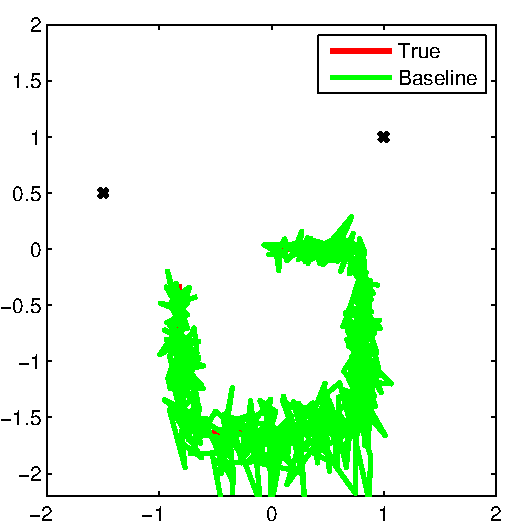
\includegraphics[width=0.7\textwidth]{ex_4_3_baseline}}                
	  \subfloat[EKF approximation]{\label{fig:ex_4_3_ekf}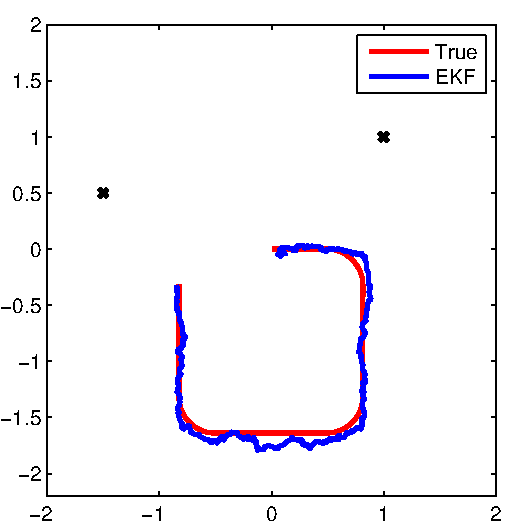
\includegraphics[width=0.7\textwidth]{ex_4_3_ekf}}
  \end{adjustwidth}
  	  \caption{The true trajectory, the baseline approximation and the EKF approximation in exercise~\ref{sec:4_3a}}
	  \label{fig:ex_4_3}
\end{figure}



\begin{table}[h]
	\centering
	\topcaption{The RMSE values in exercise \ref{sec:4_3a}}
	\begin{tabular}{c c c}
		\otoprule
		Baseline & EKF\\
		\midrule
		$1.019$ & $0.441$\\
		\bottomrule
	\end{tabular}
	\label{table:rmse4.3}
\end{table}

\clearpage


\lstinputlisting[linerange=141-182,caption={m-code in exercise~\ref{sec:4_3a}},label=lst:4_3a]{angle_ex.m}



%\bibliographystyle{plain}
%\bibliography{viitteet}
\end{document}
